\documentclass{article}
\usepackage[utf8]{inputenc}
\usepackage[a4paper, top=2cm, bottom=2cm, left=2cm, right=2cm]{geometry}
\usepackage{amsfonts}
\usepackage{amsmath}
\usepackage{amssymb}
\usepackage{amsthm}
\usepackage{esint}
\usepackage{fancyhdr}
\usepackage{enumitem}
\usepackage{amsmath}
\usepackage{amsthm}
\usepackage{amssymb}
\usepackage{mathabx}
\usepackage[linesnumbered , ruled , vlined]{algorithm2e}
\usepackage{listings}
\usepackage{xcolor}
\usepackage{floatrow}
\usepackage{graphicx}
\usepackage{fancyhdr}
\usepackage{listings}
\usepackage[hypcap=false]{caption}
\usepackage{hyperref}
\usepackage{subfig}
\usepackage{tikz}
% \usepackage{float}
\usetikzlibrary{chains,fit,shapes,automata}

\pagestyle{fancy}
\fancyhf{}
\lhead{200050154, 200050157}
\rhead{CS310}
\cfoot{\thepage}

\newcommand{\B}[1]{\textbf{#1}}
\newcommand{\I}[1]{\textit{#1}}

\title{\textbf{CS310 Lecture 14 \\ Introduction to Turing Machines}}
\author{Vedang Asgaonkar (200050154), Virendra Kabra (200050157)}
\date{28 September 2022}

\begin{document}
\begin{sloppypar}       % for overfull, etc.

    \maketitle

    \section{Recap}
    \begin{itemize}
        \item We have seen FSA and PDA, and their limitations. For example, $\{a^nb^n\ |\ n\ge1\}$ and $\{a^nb^nc^n\ |\ n\ge1\}$ cannot be expressed using FSA and PDA, respectively.
        \item Deterministic PDA (DPDA) accept all regular languages, but only a proper subset of CFLs. For instance, $\{ww^R\ |\ w\in\{0,1\}^*\}$ has no DPDA, but is context-free. In this sense, non-deterministic PDA are more powerful than DPDA.
        \item PDA with two stacks are as powerful as Turing Machines. For example, $\{a^nb^nc^n\ |\ n\ge1\}$ can be expressed as follows: Push $a$'s and $b$'s in separate stacks (ensuring that $b$'s follow $a$'s). For every $c$, pop from each stack. Accept iff both stacks are empty and the entire input string is consumed. Other data structures, such as queues, can also be used.
    \end{itemize}

    \section{Turing Machines}
    \begin{itemize}
        \item Formal notation: 7-tuple $M = (Q,\Sigma,\Gamma,\delta,q_0,B,F)$
        \begin{itemize}
            \item $Q$: Finite set of states.
            \item $\Sigma$: Finite set of input symbols.
            \item $\Gamma$: Complete set of tape symbols. That is, $\Sigma, B$, and other tape symbols.
            \item $\delta$: Transition function ($Q\times\Gamma \rightarrow Q\times\Gamma\times\{L,R\}$). This is a partial mapping. $\delta(q,X) = (p,Y,D)$, where $q,X$ are current state and tape symbol, $p,Y,D$ are next state, replacement symbol, and direction, respectively.
            \item $q_0$: Start state.
            \item $B$: Blank symbol. $B\in\Gamma, B\notin\Sigma$.
            \item $F$: Set of final/accepting states.
        \end{itemize}
        The tape is divided into \I{cells}, each holding an element of $\Gamma$. The tape can be doubly-infinite, or bounded at one end (this does not change the computational power). The \I{tape head} is always positioned at one of the tape cells.

        \item Instantaneous Description (ID): At any point, the TM can be represented as $X_1X_2\cdots X_{i-1}qX_iX_{i+1}\cdots X_n$, where
        \begin{itemize}
            \item $q$ is the current state.
            \item Tape head points to $X_i$.
            \item $X_1\cdots X_n$ is the portion of the tape between the leftmost and rightmost blank cells. If the head points to a blank cell, then some prefix or suffix of $X_1\cdots X_n$ will be blank.
        \end{itemize}
        ID's are used to describe moves of the TM. If $\delta(q,X_i) = (p,Y,L)$, then $X_1\cdots X_{i-1}qX_iX_{i+1}\cdots X_n \vdash X_1\cdots X_{i-2}pX_{i-1}YX_{i+1}\cdots X_n$. If $i=1$, we get $pBYX_2\cdots X_n$. If $i=n$ and $Y=B$, we get $X_1\cdots X_{n-2}pX_{n-1}$. $\vdash^*$ is used for zero or more moves.

        \item Example 1: $L = \{0^n1^n\ |\ n\ge1\}$
        
        \begin{minipage}{\linewidth}

            \centering

            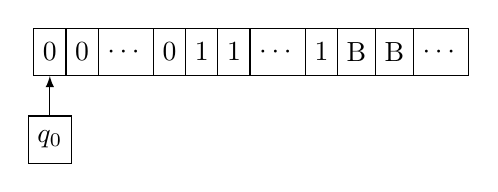
\begin{tikzpicture}

                    % https://texample.net/tikz/examples/turing-machine-2/
                    % https://tex.stackexchange.com/questions/49839/turing-machine-figure
                    % indentation [use minipage]: https://tex.stackexchange.com/questions/54448/
                    % reference: https://tex.stackexchange.com/questions/315584/
                    % new line in label: https://tex.stackexchange.com/questions/24372
                
                \edef\sizetape{0.6cm}
                \tikzstyle{tmtape}=[draw,minimum height=\sizetape,rectangle]
                
                \begin{scope}[start chain=1 going right,node distance=-0.15mm]
                    \node [on chain=1,tmtape] (input) {0};
                    \node [on chain=1,tmtape] {0};
                    \node [on chain=1,tmtape] {$\cdots$};
                    \node [on chain=1,tmtape] {0};
                    \node [on chain=1,tmtape] {1};
                    \node [on chain=1,tmtape] {1};
                    \node [on chain=1,tmtape] {$\cdots$};
                    \node [on chain=1,tmtape] {1};
                    \node [on chain=1,tmtape] {B};
                    \node [on chain=1,tmtape] {B};
                    \node [on chain=1,tmtape] {$\cdots$};
                    \node [on chain=1,tmtape,below = 0.5cm of input,align=center] (control) {$q_0$};  %Finite\\control
                \end{scope}

                \draw[-latex] (control) -- (input);
            
            \end{tikzpicture}

        \end{minipage}
        
        \begin{minipage}{\linewidth}

            \centering

            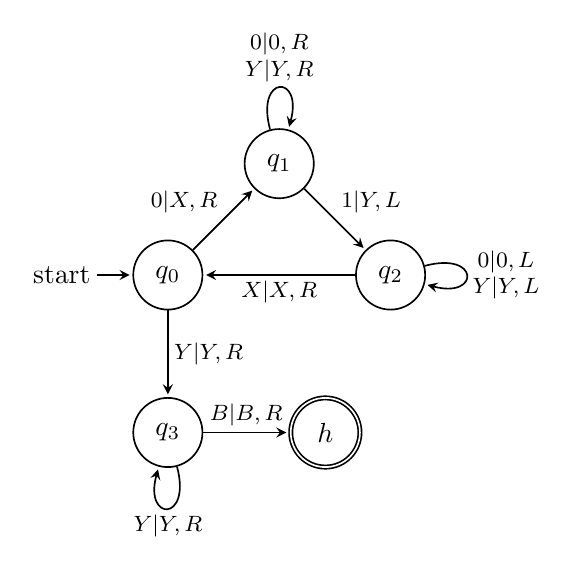
\begin{tikzpicture}[->,>=stealth,shorten >=1pt,auto,node distance=2cm,semithick,inner sep=2pt,bend angle=45]
                \node[state,initial] (0) {$q_0$};
                \node[state] (1) [above right of=0] {$q_1$};
                \node[state] (2) [below right of=1] {$q_2$};
                \node[state] (3) [below of=0] {$q_3$};
                \node[state,accepting] (halt) [right of=3] {$h$};
                \tikzstyle{every node}=[font=\footnotesize]         % for edge labels
                \path
                    (0) edge node {$0|X,R$} (1)
                        edge node {$Y|Y,R$} (3)
                    (1) edge [loop above] node[align=center] {$0|0,R$\\$Y|Y,R$} (1)
                        edge node {$1|Y,L$} (2)
                    (2) edge node {$X|X,R$} (0)
                        edge [loop right] node[align=center] {$0|0,L$\\$Y|Y,L$} (2)
                    (3) edge [loop below] node {$Y|Y,R$} (3)
                        edge node {$B|B,R$} (halt);
                    % (C) edge node {0,1,L} (D)
                        % edge [bend left] node {1,0,R} (E)
                    % (D) edge [loop below] node {1,1,R} (D)
                        % edge node {0,1,R} (A)
                    % (E) edge [bend left] node {1,0,R} (A);
            \end{tikzpicture}

            \captionof{figure}{TM for $\{0^n1^n\ |\ n\ge1\}$}
            \label{fig:1}

        \end{minipage}

        \begin{itemize}
            \item Formally, the TM is $M=(\{q_0,q_1,q_2,q_3,h\},\{0,1\},\{0,1,X,Y,B\},\delta,q_0,B,\{h\})$. $\delta$ is given by the state transitions, and $h$ is the \I{halt state}. A left-bound is assumed on the tape. As mentioned earlier, this has no effect on the computational power.
            \item Starting at the left end, the loop $q_0-q_1-q_2-q_0$ changes a $0$ to $X$, and moves right over $0$'s and $Y$'s. Then, it changes a corresponding $1$ to $Y$, and moves left over $Y$'s and $0$'s. In this process, if some other symbol is encountered, the machine `crashes'. After finding an $X$, it checks if a $0$ is present at its immediate right. If present, the entire loop repeats. Else, $M$ moves to $q_3$ (if the symbol is a $Y$). Then, after moving right over several $Y$'s, it accepts on a $B$.
            \item Note: Merging $q_0$ and $q_3$ changes the language. The resulting TM would accept strings such as $0101\notin L$ too.
            \item To accept $L\cup\{\varepsilon\}$, an additional transition $\delta(q_0,B)=(h,B,R)$ can be added.
        \end{itemize}


        % a^n b^n c^n
        \item Example 2: $L = \{a^nb^nc^n\ |\ n\ge1\}$
        
        \begin{minipage}{\linewidth}

            \centering

            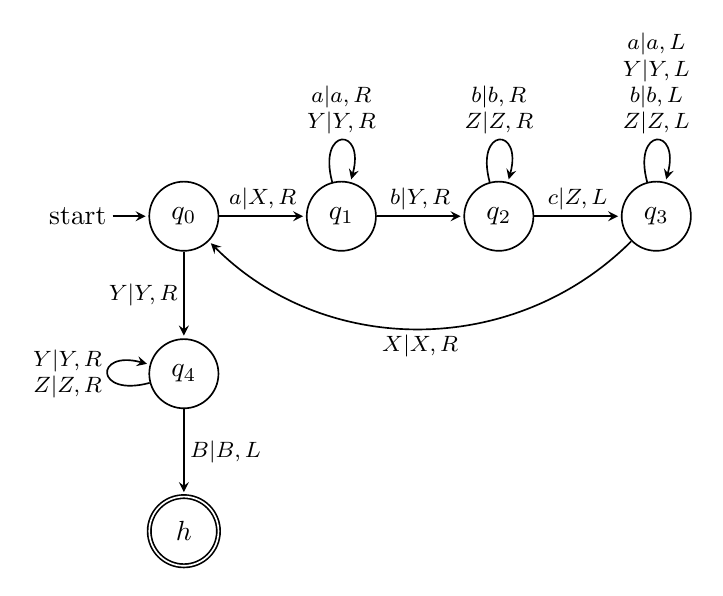
\begin{tikzpicture}[->,>=stealth,shorten >=1pt,auto,node distance=2cm,semithick,inner sep=2pt,bend angle=45]
                \node[state,initial] (0) {$q_0$};
                \node[state] (1) [right of=0] {$q_1$};
                \node[state] (2) [right of=1] {$q_2$};
                \node[state] (3) [right of=2] {$q_3$};
                \node[state] (4) [below of=0] {$q_4$};
                \node[state,accepting] (halt) [below of=4] {$h$};
                \tikzstyle{every node}=[font=\footnotesize]         % for edge labels
                \path
                    (0) edge node {$a|X,R$} (1)
                        edge node[left] {$Y|Y,R$} (4)
                    (1) edge [loop above] node[align=center] {$a|a,R$\\$Y|Y,R$} (1)
                        edge node {$b|Y,R$} (2)
                    (2) edge [loop above] node[align=center] {$b|b,R$\\$Z|Z,R$} (2)
                        edge node {$c|Z,L$} (3)
                    (3) edge [loop above] node[align=center] {$a|a,L$\\$Y|Y,L$\\$b|b,L$\\$Z|Z,L$} (3)
                        edge [bend left] node {$X|X,R$} (0)
                    (4) edge [loop left] node[align=center] {$Y|Y,R$\\$Z|Z,R$} (4)
                        edge node {$B|B,L$} (halt);
            \end{tikzpicture}

            \captionof{figure}{TM for $\{a^nb^nc^n\ |\ n\ge1\}$}
            \label{fig:2}

        \end{minipage}

        This follows from the previous example. Here, the loop $q_0-q_3-q_0$ marks corresponding input symbols with $X,Y,Z$. Then, we accept on the path $q_0-q_4-h$.

    \end{itemize}

    \newpage

    \section{Computations with Turing Machines}
    \begin{itemize}
        \item Suppose we wish to compute an $n$-ary function on a TM. The arguments (which are assumed to be integers) are provided on the tape in unary format. The unary alphabet is $\{0\}$ and we separate the arguments using $1$'s.
        \item The function's return value is written on the tape when it finishes execution.

        \item Example 1: Consider the \I{monus} function, defined as $f(x_1, x_2) = x_1\dotdiv x_2 = \max(0, x_1-x_2)$. The following machine computes this function:
        
        \begin{minipage}{\linewidth}

            \centering

            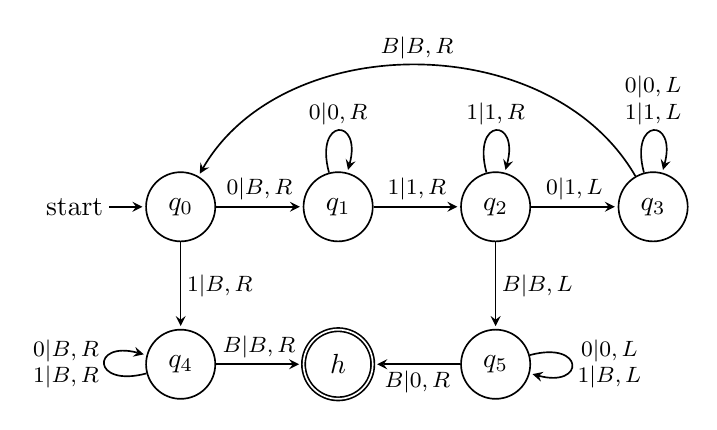
\begin{tikzpicture}[->,>=stealth,shorten >=1pt,auto,node distance=2cm,semithick,inner sep=2pt,bend angle=45]
                \node[state,initial] (0) {$q_0$};
                \node[state] (1) [right of=0] {$q_1$};
                \node[state] (2) [right of=1] {$q_2$};
                \node[state] (3) [right of=2] {$q_3$};
                \node[state] (4) [below of=0] {$q_4$};
                \node[state] (5) [below of=2] {$q_5$};
                \node[state,accepting] (halt) [right of=4] {$h$};
                \tikzstyle{every node}=[font=\footnotesize]
                \path
                    (0) edge node {$0|B,R$} (1)
                        edge node {$1|B,R$} (4)
                    (1) edge [loop above] node {$0|0,R$} (1)
                        edge node {$1|1,R$} (2)
                    (2) edge [loop above] node {$1|1,R$} (2)
                        edge node {$0|1,L$} (3)
                        edge node {$B|B,L$} (5)
                    (3) edge [loop above] node[align=center] {$0|0,L$\\$1|1,L$} (3)
                        edge [bend right=60] node[above] {$B|B,R$} (0)
                    (4) edge [loop left] node[align=center] {$0|B,R$\\$1|B,R$} (4)
                        edge node {$B|B,R$} (halt)
                    (5) edge [loop right] node[align=center] {$0|0,L$\\$1|B,L$} (5)
                        edge node {$B|0,R$} (halt);
            \end{tikzpicture}

            \captionof{figure}{TM for \I{monus} function}
            \label{fig:3}

        \end{minipage}

        % \begin{center}
        %     \ffigbox [ 1 \textwidth ]{ \caption{monus function} } { \includegraphics [ width =1 \textwidth ] {monus.jpeg}}   
        % \end{center}

        This machine cancels out $0$'s from the arguments one by one, till one of them runs out (this is the loop $q_0-q_3-q_0$). The left branch $q_0-q_4-h$ deals with $x1\le x2$, resulting in a blank tape, while $q_2-q_5-h$ deals with $x_1>x_2$. In either case, $M$ halts with $0^{x_1\dotdiv x_2}$ on the tape, blanking out everything else.

        \item Example 2: Consider a TM that performs addition on positive numbers $x_1$ and $x_2$. To do this, we simply modify the separator $1$ to $0$, and blank out the last $0$. This results in a block of $x_1+x_2$ contiguous $0$'s.
        
        \begin{minipage}{\linewidth}

            \centering

            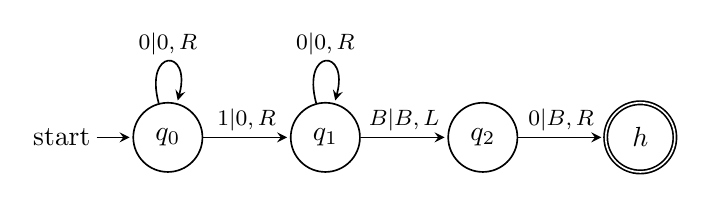
\begin{tikzpicture}[->,>=stealth,shorten >=1pt,auto,node distance=2cm,semithick,inner sep=2pt,bend angle=45]
                \node[state,initial] (0) {$q_0$};
                \node[state] (1) [right of=0] {$q_1$};
                \node[state] (2) [right of=1] {$q_2$};
                \node[state,accepting] (halt) [right of=2] {$h$};
                \tikzstyle{every node}=[font=\footnotesize]
                \path
                    (0) edge [loop above] node {$0|0,R$} (0)
                        edge node {$1|0,R$} (1)
                    (1) edge [loop above] node {$0|0,R$} (1)
                        edge node {$B|B,L$} (2)
                    (2) edge node {$0|B,R$} (halt);
            \end{tikzpicture}

            \captionof{figure}{TM for unary adder}
            \label{fig:4}

        \end{minipage}

        % \begin{center}
        %     \ffigbox [ 1 \textwidth ]{ \caption{unary adder} } { \includegraphics [ width =1 \textwidth ] {add.jpeg}}   
        % \end{center}
        
    \end{itemize}


    \section{References}
    \begin{itemize}
        \item Section 8.2 of Hopcroft, Motwani, Ullman.
    \end{itemize}

\end{sloppypar}
\end{document}